\documentclass{../../text-style}

\texttitle{Лекция 8/Практика 7: Поведенческие шаблоны}

\begin{document}

\maketitle
\thispagestyle{empty}

\section{Паттерн <<Команда>>}

\subsection{Мотивирующий пример}

Положим, у нас всё ещё есть текстовый редактор, над которым мы как бы работаем на протяжении всех лекций про паттерны. Теперь мы хотим сделать пользовательский интерфейс с командами, выполняющими всякие действия типа сохранения и загрузки файла, смены параметров шрифта и т.п. Причём, как и у всех приличных текстовых редакторов, у нас есть палитра инструментов, основное меню приложения, горячие клавиши --- и это на самом деле несколько способов вызвать одно и то же действие. Захардкодить в каждом пункте меню, что по его активации вызывается соответствующий метод бизнес-логики кажется плохой идеей --- получится, что элементы управления должны будут знать о классах бизнес-логики. Окей, мы можем применить паттерн <<Наблюдатель>> подписывать объект бизнес-логики на события от элементов управления, и это будет уже лучше, но тут мы вспомним, что надо ведь ещё поддержать undo/redo, и делать это в самой бизнес-логике нам бы очень не хотелось...

Решение --- обернём действие в объект: 

\begin{center}
    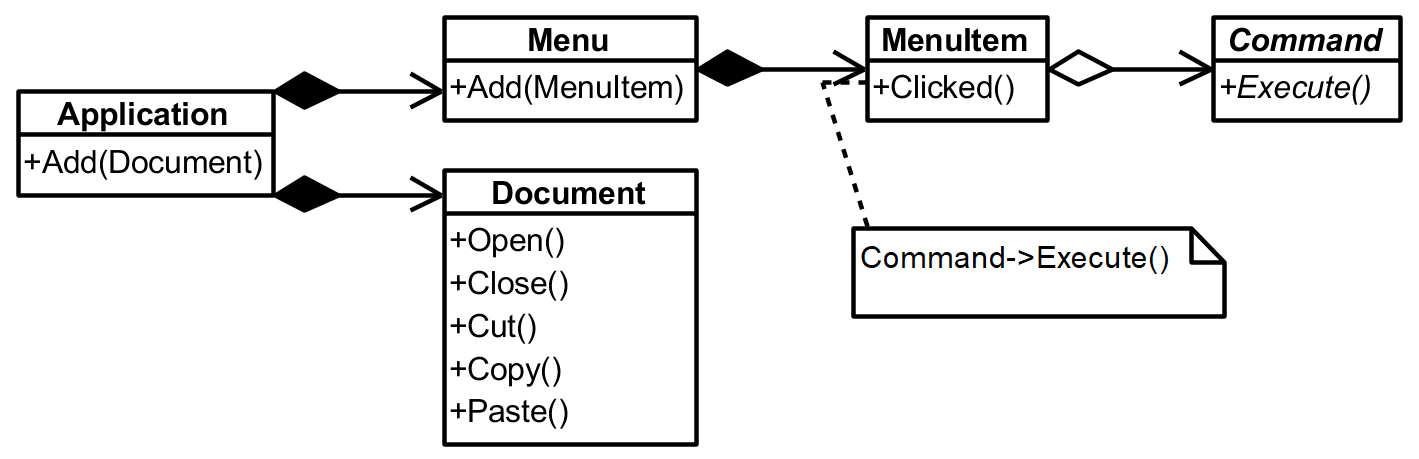
\includegraphics[width=0.9\textwidth]{commandExample.png}
\end{center}

Теперь сама команда --- это метод Execute() класса Command, и только он знает про бизнес-логику, которая реально исполняет команду (в данном примере она размещена в классе Document). Мы можем теперь создать объект Command и отдать его в главное меню, кнопке на палитре инструментов, менеджеру хоткеев и т.п., один и тот же объект, который исполняет одно действие. Таким образом, никто из потенциальных инициаторов команды не будет знать про то, что она делает (они видят только по сути интерфейс с одним методом). Это позволит легко менять команды разным элементам управления, и сделать их полностью независимыми от бизнес-логики. При этом команда может хранить в себе состояние, нужное для отмены операций.

Например, команда вставки:

\begin{center}
    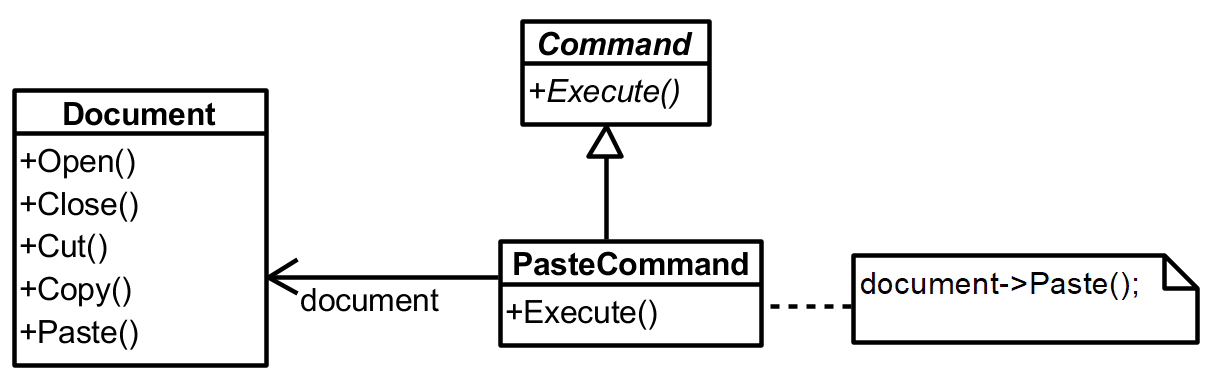
\includegraphics[width=0.8\textwidth]{pasteCommand.png}
\end{center}

PasteCommand реализует интерфейс Command очень простым образом --- она просто вызывает метод Paste() у класса с бизнес-логикой и больше ничего интересного не делает.

Или команда открытия документа:

\begin{center}
    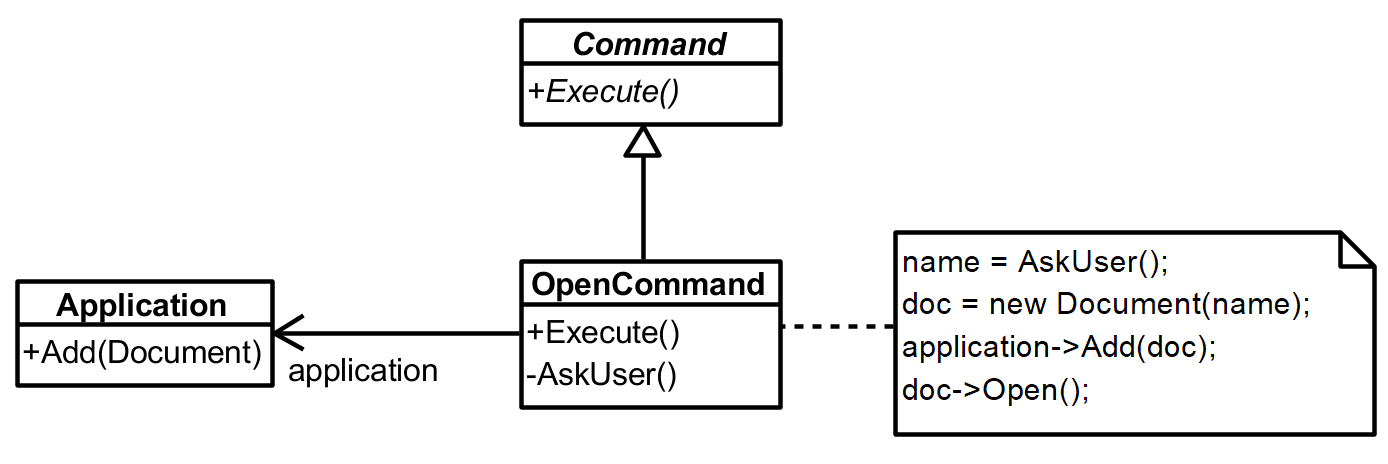
\includegraphics[width=0.8\textwidth]{openDocumentCommand.png}
\end{center}

Она уже сама содержит в себе логику взаимодействия с пользователем: сначала запрашивает у пользователя имя файла, потом создаёт документ, потом регистрирует его в приложении и открывает. Обратите внимание, команда, хоть и содержит нетривиальную логику, не реализует бизнес-логику работы с документами, она лишь взаимодействует с пользователем и <<оркестрирует>> основные классы системы.

А ещё команда может быть составной:

\begin{center}
    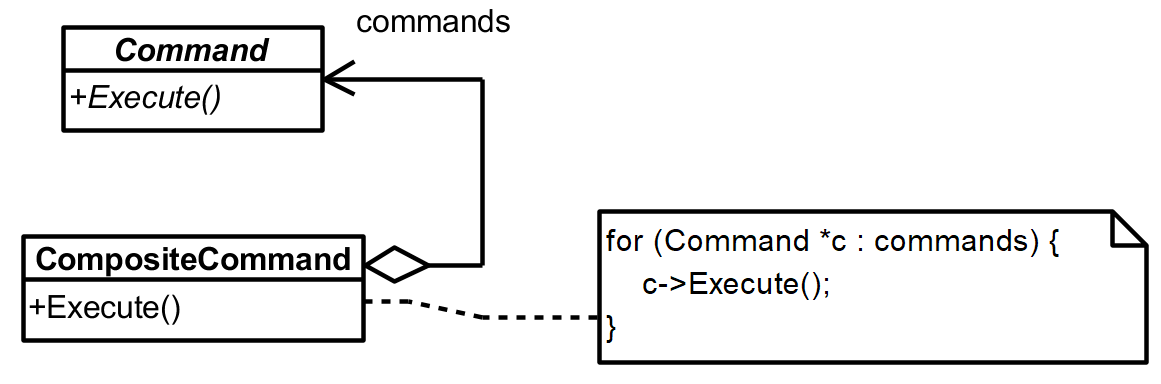
\includegraphics[width=0.7\textwidth]{compositeCommand.png}
\end{center}

Это полезно, когда один инициатор действия должен инициировать сразу несколько действий. Это позволяет легко поддержать макросы, но также полезно и для обычных команд: например, по нажатию на Enter в большинстве сред разработки выполняется переход на новую сроку и вставка отступа. В некоторых средах, если последовательно отменить эти действия, видно, что одно нажатие на Enter на самом деле спровоцировало два отдельных действия, с независимой отменой.

\subsection{Команда (Command), общая структура}

Идеи выше обобщаются до паттерна <<Команда>> с довольно нетривиальной структурой:

\begin{center}
    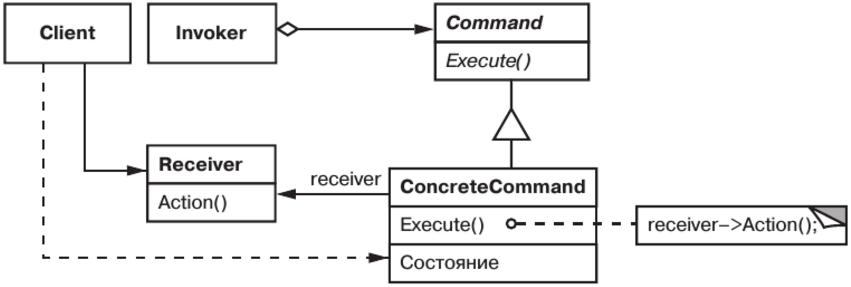
\includegraphics[width=0.8\textwidth]{command.png}
    \attribution{Э. Гамма и др., Приемы объектно-ориентированного проектирования}
\end{center}

Client --- это тот, кто пользуется всеми командами, как правило, это само приложение в целом (например, его функция main или аналог). Client создаёт классы, которые будут отвечать за бизнес-логику, стоящую за командами (класс Receiver), создаёт инициаторов действий (класс Invoker), создаёт конкретные команды, даёт им ссылки на их Receiver-ов и отдаёт Invoker-ам то, что получилось. Дальше, когда пользователь взаимодействует с приложением, он вызывает Invoker, тот вызывает виртуальный метод Execute() у Command, тот делает что-то полезное, вызывая Receiver:

\begin{center}
    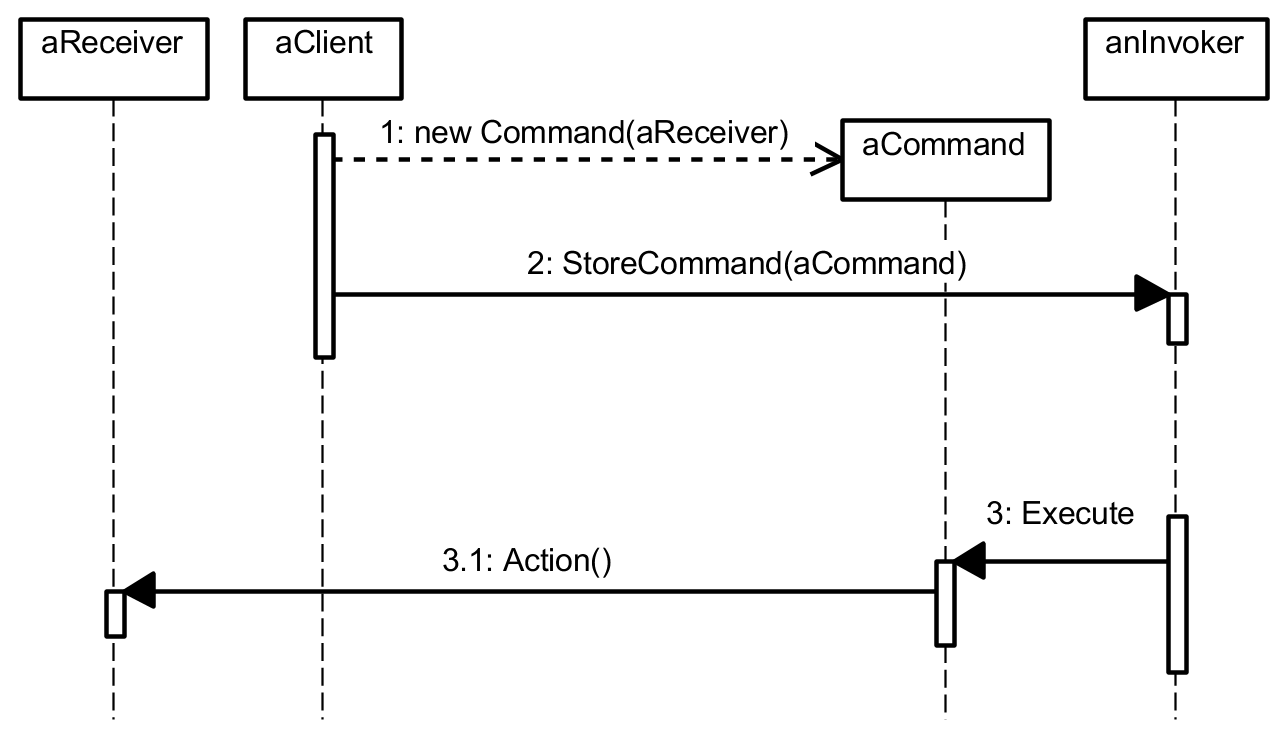
\includegraphics[width=0.8\textwidth]{commandSequence.png}
\end{center}

В нашем примере с редактором Client --- это Application, Receiver --- это Document, Invoker --- это MenuItem, а Command, кажется, очевидно кто.

Применяется этот паттерн, когда надо уметь работать с запросами как с объектами: хранить запросы, ставить в очередь на обработку, исполнять в произвольное время (ну, в большинстве случаев не в произвольное, а как будем готовы) и т.д. При этом команда --- это ещё и способ параметризовать объект исполняемым действием (то есть имеет <<встроенный>> паттерн <<Стратегия>>, Command же по сути Strategy для Invoker-а). Если немного расширить предложенную схему, легко поддержать отмену операций --- команда может хранить состояние, и если её не выкидывать после исполнения, может быть использована для возврата системы в вид, в котором она была до исполнения команды.

Архитектурно паттерн <<Команда>> тоже хорош, поскольку позволяет структурировать взаимодействие с пользователем. Если он последовательно применяется, то через команды проходит всё взаимодействие с пользователем, что позволяет иметь одно выделенное место в структуре системы, куда можно добавить логирование, валидацию и т.п. Кроме того, возможность собирать из простых команд составные (хоть полноценный паттерн <<Компоновщик>>) позволяет структурировать систему, собирая сколь угодно сложное взаимодействие с пользователем из элементарных операций.

В реальной жизни паттерн команда в том или ином виде есть в любой нормальной оконной библиотеке, так что непременно встретится на практике.

\subsection{Детали реализации}

С точки зрения реализации паттерн <<Команда>> предлагает на выбор массу архитектурных вариантов. Во-первых, насколько <<умной>> должна быть команда:

\begin{itemize}
    \item команда может вообще ничего не знать про логику работы приложения, да даже и про Receiver-а знать только то, что он есть и надо его дёрнуть, когда команду активируют;
    \item команда может выполнять всю полезную работу сама и никакой Receiver ей вообще не нужен;
    \item возможны и встречаются на практике также все промежуточные варианты.
\end{itemize}

<<Глупые>> команды хороши тем, что всю машинерию, связанную с командами, можно реализовать в библиотеке, и сами команды очень просты, выступая по сути исключительно методом связи Invoker-а и Receiver-а. Зато всю логику повторения и отмены операций, логирования и т.п. надо будет писать в Receiver-е, что для сложных систем может быть плохой идеей.

<<Умные>> команды могут быть идеальны, если всё приложение строится вокруг пользовательского интерфейса (например, штука для показа прогноза погоды или постов в Твиттере). Структурирование бизнес-логики по командам в этом случае может быть хорошей идеей с точки зрения архитектуры.

Однако команды, хоть и не привязаны к конкретным элементам управления, всё-таки слишком специфичны для приложения, поэтому переиспользовать их для другой задачи в рамках той же предметной области может быть проблематично. Поэтому часто используют не очень умные, но и не очень глупые команды --- команды, которые знают про логику взаимодействия с пользователем и сценарии использования конкретного приложения, но используют для своего исполнения объекты, моделирующие предметную область (они вообще ни о чём, кроме предметной области, знать не должны, поэтому великолепно переиспользуемы). В какой степени используют --- вопрос, на который приходится отвечать для каждой конкретной системы, так что можно сказать, что <<глупость-умность>> --- это шкала, причём шкала без дискретных значений.

Следующий архитектурный вопрос касается реализации отмены и повторения операций (Undo-Redo в англоязычной литературе). Делается это в целом довольно просто: заводятся два стека, Undo-стек и Redo-стек. Команде в дополнение к методу Execute() делают ещё метод Undo(). Когда команду исполняют впервые, вызывается её метод Execute() и команда кладётся на Undo-стек. Если пользователь хочет отменит операцию, с вершины Undo-стека снимается команда, вызывается её метод Undo() и команда перекладывается на Redo-стек. Если пользователь передумал отменять команду и хочет вернуть всё как было, команда снимается с вершины Redo-стека, снова вызывается её метод Execute() и команда кладётся на Undo-стек. Если исполняется какая-то новая команда (не с Undo- или Redo-стека), Redo-стек очищается. 

Обычно все эти стеки и механизм перекладывания команд туда-сюда реализуется в отдельном классе (обычно Controller), он же и исполняет команды --- то есть Invoker не вызывает на самом деле сам Execute(), он просто вызывает контроллер, отдавая ему активированную команду.

Собственно, архитектурный вопрос в том, как реализовать операцию Undo() в команде. Это опять зависит от конкретной задачи. Можно хранить в команде всё состояние системы целиком, а в Undo() просто возвращать систему в исходное состояние. Можно хранить дельту относительно предыдущего состояния и вычислять обратное преобразование, которое отменит команду (например, в текстовом редакторе команде добавления буквы в текст достаточно просто запомнить позицию добавленной буквы, чтобы в Undo() её удалить --- но помните, что при повторном вызове Execute() нам надо иметь возможность повторить команду, так что надо запомнить и позицию, и саму букву).

Выше говорилось, что, мол, есть команда, это один объект, который раздаётся разным Invoker-ам, а тут ещё, оказывается, он хранится в Undo- или Redo-стеке и запоминает состояние. А что будет, если одну и ту же команду активировали дважды? Да, это проблема, и если команда мутабельна (то есть правда хранит состояние), перед тем, как её исполнить в первый раз, надо её скопировать. Может помочь паттерн <<Прототип>>.

Также могут быть полезны искусственные команды --- то есть команды, которые не активируются ничем из пользовательского интерфейса, а добавляются в контроллер другими классами системы. Это при неаккуратной реализации может удивить пользователя (когда он сможет отменить то, чего сам никогда не делал), но это решается наличием в команде одного булевого флага, что она искусственная. Также применяются и композитные команды, которые позволяют одно действие из пользовательского интерфейса исполнить с помощью нескольких элементарных команд. Откатывать лучше всю композитную команду целиком, поэтому желательно класть на стек именно её, а не её подчинённые команды.

Паттерн <<Команда>> в плане отката операций хорошо комбинируется с паттерном <<Хранитель>>. <<Хранитель>> может сделать слепок состояния системы (или части состояния, необходимой для восстановления), отдать его команде, а потом, при отмене команды, восстановить состояние системы из слепка. Команда в этом случае выступает в роли Caretaker-а из паттерна <<Хранитель>> (про который чуть позже).

Вот пример <<глупой>> команды из реального мира, оконной библиотеки для C++ со звучным названием Qt\footnote{в C++ много чего называется совершенно непроизносимо, хотя конкретно Qt читается как <<кьют>>, созвучно английскому <<cute>>, <<милый>> --- или \emph{они} хотят заставить нас в это поверить.}:

\begin{minted}{c++}
const QIcon openIcon = QIcon(":/images/open.png");
QAction *openAct = new QAction(openIcon, tr("&Open..."), this);

openAct->setShortcuts(QKeySequence::Open);
openAct->setStatusTip(tr("Open an existing file"));

connect(openAct, &QAction::triggered, this, &MainWindow::open);

fileMenu->addAction(openAct);
fileToolBar->addAction(openAct);
\end{minted}

Команда тут --- это класс QAction. Ей при создании выдают иконку, текст названия команды (используется функция tr, возвращающая перевод (<<translation>>) строки для текущей локали), задаётся горячая клавиша (привязанная к константе, соответствующей Ctrl-O или чему-то такому в зависимости от операционной системы), всплывающая подсказка. Дальше с помощью функции connect и Qt-шной магии (весьма продвинутой, к слову --- в Qt есть собственный препроцессор и кодогенератор, запускающийся до основной компиляции) событие triggered команды связывается с обработчиком open класса MainWindow. MainWindow в данном случае выступает в роли Receiver-а из паттерна. Дальше команда отдаётся основному меню приложения и панели инструментов, которые используют иконку и текст команды, чтобы отобразить их на кнопке и в пункте меню соответственно. Теперь, когда пользователь активирует команду (например, нажав хоткей или кликнув на кнопку на панели инструментов), команда активирует событие triggered, что приведёт к вызову метода open у объекта MainWindow. 

Тут команда вообще просто библиотечный класс и всю работу делает Receiver. Пользоваться такой командой очень удобно при разработке пользовательских интерфейсов, однако для организации обработки запросов глубоко внутри приложения такая реализация не годится (иконка нужна, например). Автору пришлось писать свой аналог вручную, чтобы использовать команды для обработки заданий в глубине приложения.

\section{Паттерн <<Хранитель>>}

\subsection{Мотивирующий пример}

В качестве мотивирующего примера вспомним про отмену и повторение операций, которые обсуждались в паттерне <<Команда>>. Допустим, мы делаем векторный графический редактор и хотим уметь отменять перемещение фигур, которые могут быть связаны друг с другом. Простая реализация, где у каждой фигуры есть координаты, и отмена команды просто возвращает старые координаты перемещённой фигуре, может столкнуться с таким казусом:

\begin{center}
    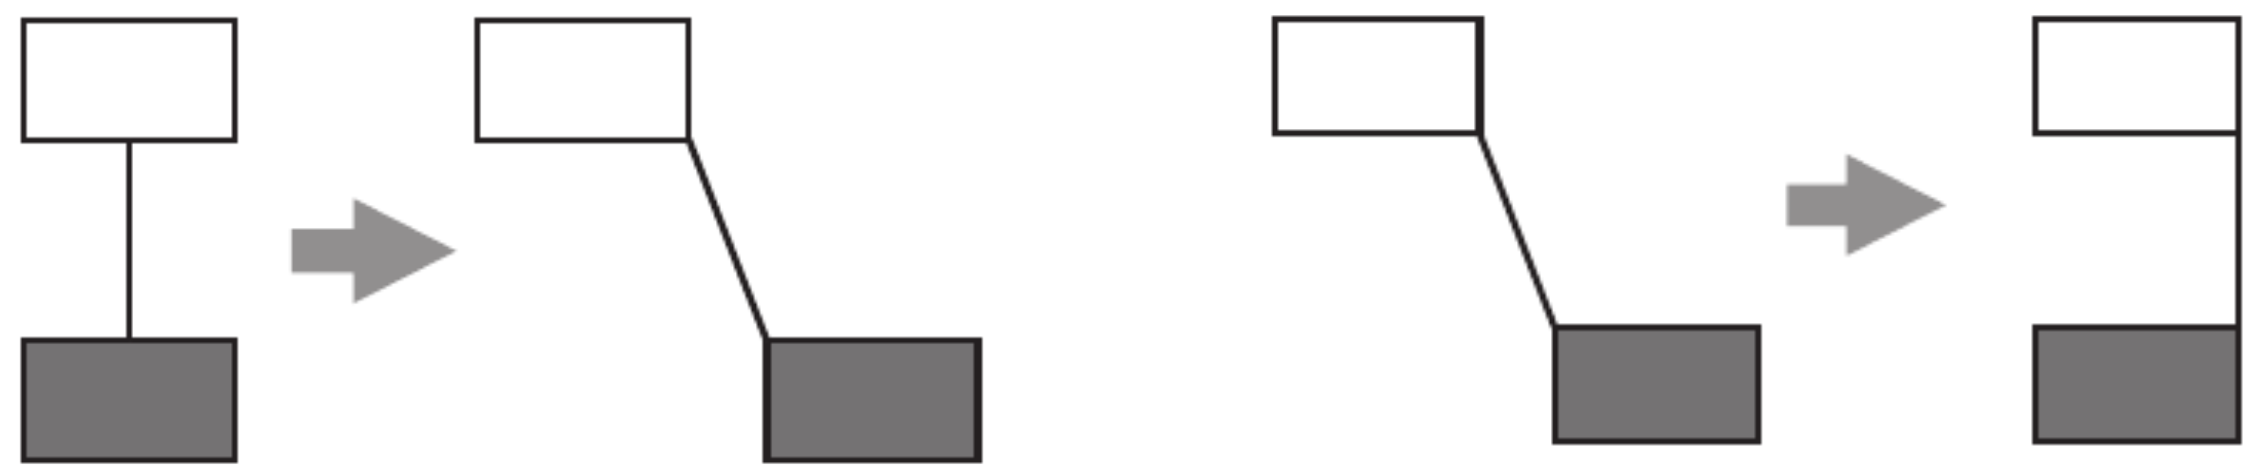
\includegraphics[width=0.8\textwidth]{mementoMotivation.png}
    \attribution{Э. Гамма и др., Приемы объектно-ориентированного проектирования}
\end{center}

Тут фигура честно вернулась в исходное положение, но связь подумала, что фигура просто переместилась, и прицепилась не к тем точкам, что были изначально.

Паттерн <<Хранитель>> описывает более-менее общее решение по хранению всякой информации о состоянии объекта так, чтобы его можно было потом восстановить, и, главное, так, чтобы детали этого состояния не раскрывались сторонним объектам. Например, у нас команда для операции отмены вынуждена знать координаты фигуры, а потом ещё координаты всех связей фигуры, а потом окажется, что и ещё что-то (если вдруг отработал алгоритм автоматического размещения, команде надо знать про координаты вообще всех объектов на сцене). Команде этого всего знать не надо на самом деле, она должна просто получить некое состояние на хранение, а когда ей вызовут Undo(), выдать сохранённое состояние фигуре (или сцене), чтобы те уже сами из него восстановили всё как было. Вот, собственно, этим паттерн <<Хранитель>> и занимается.

\subsection{Хранитель (Memento), общая структура}

Общая структура паттерна такова:

\begin{center}
    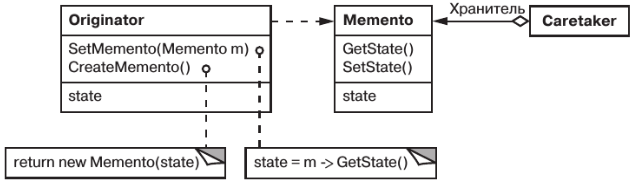
\includegraphics[width=0.7\textwidth]{memento.png}
    \attribution{Э. Гамма и др., Приемы объектно-ориентированного проектирования}
\end{center}

Originator --- это тот, кто хочет сохранить своё состояние и иметь возможность восстановиться из сохранённой копии. Memento --- это, собственно, сохранённое состояние. Caretaker --- это тот, кто состояние хранит, но не хочет (и не может) лезть внутрь. В нашем примере Caretaker --- это команда, Originator --- это фигура, а Memento --- это класс, прячущий у себя внутри координаты и фигуры, и линий, и всего, что надо.

Когда Caretaker-у нужно сохранить состояние Originator-а, он вызывает метод CreateMemento() и получает некий объект, про который сам Caretaker знает только то, что он есть (state и методы по его управлению он не видит). Когда надо восстановить состояние Originator-а, Caretaker вызывает его метод SetMemento(), Originator (зная конкретный тип Memento) пользуется GetState(), чтобы достать из Memento данные и положить их в свой state.

\subsection{Детали реализации}

В плане реализации это очень простой паттерн, но требующий языковой поддержки. В C++, например, Memento можно сделать friend-классом для Originator-а, в C\# вложенным классом в Originator, в Java --- статическим вложенным классом. В любом случае, нам нужен механизм, который бы позволял Memento иметь <<широкий>> интерфейс для Originator и <<узкий>> для всех остальных объектов. Чаще всего это требует, чтобы CreateMemento() возвращал абстрактный класс без внутренней структуры (например, Object), а SetMemento() преобразовывал его к нужному типу.

Ещё Memento не обязан хранить всё состояние Originator-а, он может хранить только дельту относительно предыдущего состояния (как бы в обратную сторону, чтобы по текущему можно было получить предыдущее). Тогда, чтобы откатиться к произвольному состоянию, надо иметь список Memento и последовательно их применять. Это экономнее в плане памяти, но гораздо хлопотнее в плане реализации. Например, системы контроля версий, можно сказать, используют такой подход.

\section{Паттерн <<Состояние>>}

\subsection{Мотивирующий пример}

На сей раз положим, что нам внезапно надо реализовать сетевой стек операционной системы. У нас есть класс TcpConnection, с методами открытия, закрытия и подтверждения, и он может находиться в трёх состояниях: соединение установлено, ожидаем соединения, соединение закрыто. Рабоче-крестьянская реализация предполагает наличие переменной-состояния в TcpConnection, по которой в каждом методе делается switch --- и, например, если мы пытаемся вызвать Open() для уже открытого соединения, то ничего не делаем. Но, как мы знаем, если у нас много где разные действия выполняются в зависимости от значения какой-то переменной, то это code smell <<тэг типа>> и его можно заменить на иерархию наследования. Так получаем уже почти паттерн <<Состояние>>:

\begin{center}
    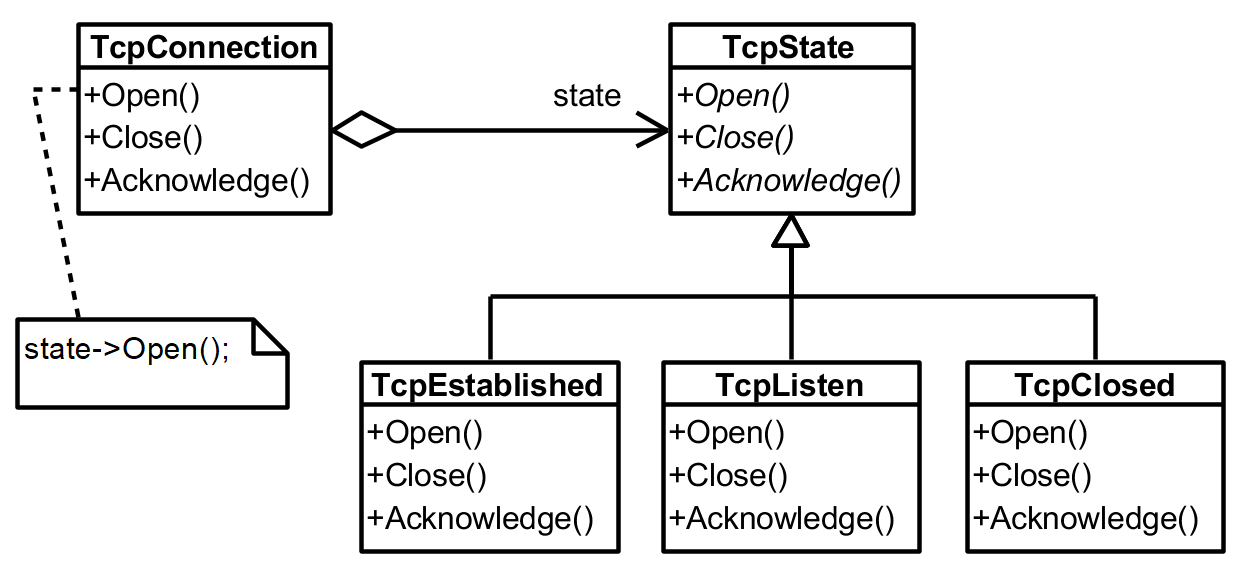
\includegraphics[width=0.75\textwidth]{stateExample.png}
\end{center}

Внешне это очень похоже на паттерн <<Стратегия>> --- есть контекст (TcpConnection), который делегирует свои основные действия объекту-состоянию (например, TcpEstablished), который их и выполняет. И в зависимости от того, в каком состоянии мы находимся, TcpConnection работает по-разному, причём переключение состояний незаметно для клиента --- он просто вызывает методы TcpConnection и не знает, что там происходит внутри. Важное отличие от <<Стратегии>> в том, что TcpConnection может переходить из состояния в состояние сам, и паттерн на самом деле определяет, как это реализуется, тогда как в <<Стратегии>> требуется участие клиента для смены стратегии. То есть <<Состояние>> можно понимать как некоторую специализированную <<Стратегию>> плюс возможность автоматически переключать поведение.

\subsection{Состояние (State), общая структура}

Общая структура паттерна такова:

\begin{center}
    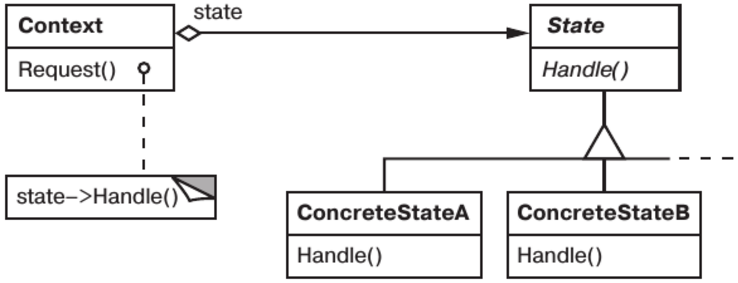
\includegraphics[width=0.6\textwidth]{state.png}
    \attribution{Э. Гамма и др., Приемы объектно-ориентированного проектирования}
\end{center}

Клиент пользуется объектом класса Context, который делегирует запрос одному из наследников класса (чаще интерфейса) State, при этом либо в Context, либо в наследниках State определяется механизм перехода из состояния в состояние. Таким образом, несмотря на то, что Context остаётся одним объектом, с точки зрения клиента всё выглядит так, будто он динамически меняет свой класс во время выполнения (как будто его методы виртуальные и у него меняется тип времени выполнения в зависимости от ситуации). Языки со строгой типизацией такого для обычных классов не позволяют, а паттерн <<Состояние>> позволяет добиться такой вот симуляции динамической типизации, что иногда бывает полезно.

Применяется этот паттерн тогда, когда поведение объекта зависит от его состояния, которое может меняться во время выполнения --- вот, например, сетевые подключения, или на самом деле все системы, выражающиеся в терминах конечных автоматов (а это большинство реактивных систем, начиная от дверного замка, заканчивая робототехническим комплексом или ИИ в компьютерных играх). Паттерн <<Состояние>> также идеален для реализации <<вручную>> конечных автоматов. Ну и в чисто прагматических целях минимизации switch, if-ов и т.п., особенно если класс явно хранит что-то, похожее на состояние, паттерн может быть полезен.

Преимущества его применения (по сравнению с другими способами реализации конечных автоматов) в том, что действия в каждом состоянии инкапсулированы в отдельный класс, так что каждое состояние легко сопровождать, да и добавлять состояния несложно. И переходы между состояниями делаются явными, что упрощает дизайн автомата. Для применений, требующих скорости работы, однако, такой подход используется редко --- например, в лексических анализаторах скорее сгенерированные таблицы переходов, они при аккуратной реализации работают в разы быстрее (что неудивительно, нет затрат на виртуальные вызовы и перенаправление запросов).

\subsection{Детали реализации}

Самое интересное при реализации паттерна --- это переходы между состояниями. Их можно делать в Context (то есть сам автомат управляет переходами) или в конкретных State (то есть каждое состояние знает, какое должно быть следующим при каком входе). Делают и так и так. Первый способ проще в плане управления состояниями (понятно, когда их создавать и удалять), и удобен тем, что есть центральное место, которое реализует логику переходов. И, кстати, логика эта может быть реализована в виде таблицы переходов --- отображения текущего состояния и входного сигнала в следующее состояние. При таком подходе, правда, сложно реализовать действие при переходе, поэтому этот способ довольно ситуационный. Второй способ --- когда само состояние возвращает при вызове действия следующее состояние --- в этом плане более гибок, но тогда логика переходов размазана по нескольким классам и в ней легко запутаться.

Ещё возникает вопрос с созданием и удалением объектов-состояний. Часто состояний немного, так что нет ничего плохого в том, чтобы создать из раз и навсегда, хранить в Context и отдавать друг другу, чтобы они знали, куда переходить. Но бывают и большие автоматы (из миллионов состояний --- надеемся, что по логике почти одинаковых), для них, возможно, более правильно было бы создавать следующее состояние при переходе в него из текущего, и удалять текущее. Но делать это надо аккуратно, чтобы не удалить состояние до того, как оно создало следующее (ошибки типа delete this;, например, иногда встречаются в коде на C++).

Ещё состояния часто могут быть разделяемыми между несколькими автоматами, особенно если не содержат никаких данных. Паттерны <<Пул объектов>> или <<Приспособленец>> помогут управлять разделяемыми состояниями. С другой стороны, обычно овчинка выделки не стоит, но ситуации бывают разные (например, некоторые алгоритмы распознавания предполагают создание нового автомата на каждый входной символ, так что легко получить миллион автоматов из нескольких сотен состояний --- там этот приём может быть полезным).

\section{Задача на практику}

Уточнить модель компьютерной игры Roguelike, используя паттерны:

\begin{enumerate}
    \item <<Команда>> для поддержки взаимодействия с пользователем --- пользовательский интерфейс не имеет права сам дёргать бизнес-логику, он может только запускать команды;
    \item <<Хранитель>> для поддержки сохранения/загрузки игры --- положим, сохранение сериализуется в, скажем, protobuf, и нам надо аккуратно реализовать модель сериализации для нашей системы;
    \item <<Состояние>> для динамического переключения поведения мобов:
    \begin{itemize}
        \item мобы с низким здоровьем должны переключаться в трусливый режим и убегают от игрока;
        \item по мере восстановления здоровья переходить в исходный;
        \item это можно понимать как то, что <<Состояние>> выбирает стратегию поведения моба, а паттерн <<Стратегия>> с предыдущего занятия отвечает за тактику. То есть состояние говорит <<атакуй>>, стратегия говорит, в какую сторону перемещаться, чтобы атаковать.
    \end{itemize}
\end{enumerate}

\end{document}